\documentclass[a4paper,12pt]{article}
\usepackage[utf8]{inputenc}
\usepackage[spanish]{babel}
\usepackage{color}
\usepackage{parskip}
\usepackage{graphicx}
\usepackage{multirow}
\usepackage{listings}
\usepackage{vmargin}
\usepackage{datetime}
\newdate{date}{12}{10}{2017}
\graphicspath{ {imagenes/} }
\definecolor{mygreen}{rgb}{0,0.6,0}
\definecolor{lbcolor}{rgb}{0.9,0.9,0.9}
\usepackage{epstopdf}
\usepackage{float}


\setpapersize{A4}
\setmargins{2.5cm}       % margen izquierdo
{1.5cm}                        % margen superior
{16.5cm}                      % anchura del texto
{23.42cm}                    % altura del texto
{10pt}                           % altura de los encabezados
{1cm}                           % espacio entre el texto y los encabezados
{0pt}                             % altura del pie de página
{2cm}     

\lstset{
%backgroundcolor=\color{lbcolor},
    tabsize=4,    
%   rulecolor=,
    language=[GNU]C++,
        basicstyle=\tiny,
        aboveskip={1.5\baselineskip},
        columns=fixed,
        showstringspaces=false,
        extendedchars=false,
        breaklines=true,
        prebreak = \raisebox{0ex}[0ex][0ex]{\ensuremath{\hookleftarrow}},
        frame=single,
        showtabs=false,
        showspaces=false,
        showstringspaces=false,
        identifierstyle=\ttfamily,
        keywordstyle=\color[rgb]{0,0,1},
        commentstyle=\color[rgb]{0.026,0.112,0.095},
        stringstyle=\color{red},
        numberstyle=\color[rgb]{0.205, 0.142, 0.73},
%        \lstdefinestyle{C++}{language=C++,style=numbers}’.
}


\begin{document}
\title{Tarea de Laboratorio 1}
\author{
Christofer Fabián Chávez Carazas \\
\small{Universidad Nacional de San Agustín de Arequipa} \\
\small{Escuela Profesional de Ciencia de la Computación} \\
\small{Compiladores}
}
\date{\displaydate{date}}

\maketitle

El objetivo de la práctica es recordar las formas de implementar una máquina de estados. Para los programas que siguen a continuación,
el fin de cadena está simbolizado por el caracter '\#'

\begin{enumerate}
 \item \textbf{Mediante un diagrama de transiciones}
 
\begin{lstlisting}
#include <iostream>
#include <cctype>
#include <clocale>

using namespace std;

int main(){
	try{
		int estado = 1;
		char c;
		cin>>c;
		while(c != '#'){
			switch(estado){
				case 1: 
					if(isalpha(c)) estado = 3;
					else if (isdigit(c)) estado = 2;
					else throw((int) 1);
					break;
				case 2: throw((int) 2);
				case 3:
					if(isalpha(c)) estado = 3;
					else if (isdigit(c)) estado = 3;
					else throw((int) 3);

			}
			cin>>c;
		}
		if(estado != 3) throw((int) 4);
		cout<<"OK..."<<endl;
	}
	catch(int e){
		switch(e){
			case 1: cout<<"Simbolo no reconocido"<<endl; break;
			case 2: cout<<"Al comenzar con un dígito debe ser el único"<<endl; break;
			case 3: cout<<"Simbolo no reconocido"<<endl; break;
			case 4: cout<<"Identificador no reconocido"<<endl; break;
		}
	}
}
\end{lstlisting}

\textbf{Resultados:}

\begin{figure}[H]
 \centering
 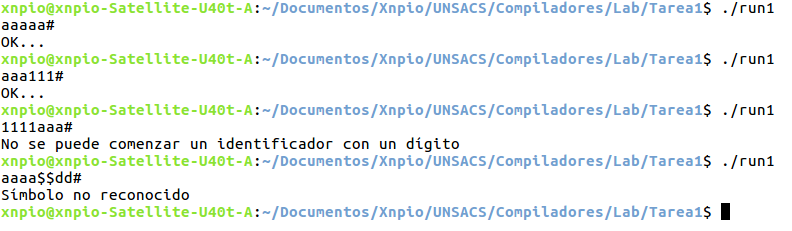
\includegraphics[scale = 0.5]{1.png}
\end{figure}


\item \textbf{Mediante una tabla de transiciones:}

\begin{lstlisting}
#include <iostream>
#include <vector>
#include <cctype>
#include <clocale>

using namespace std;

enum Tipos {LETRA, DIGITO, FDC};

vector<vector<int>> tabla = {{2,1,-1},{-1,-1,-1},{2,2,-2}};

int main(){
	try{
		int estado = 0;
		int entrada = -1;
		char c;
		cin>>c;
		while(true){
			if(c == '#') entrada = FDC;
			else if(isalpha(c)) entrada = LETRA;
			else if(isdigit(c)) entrada = DIGITO;
			else throw((int) 2);
			estado = tabla[estado][entrada];
			if(estado == -1) throw((int) 1);
			if(estado == -2){
				cout<<"OK..."<<endl;
				break;
			}
			cin>>c;
		}
	}
	catch(int e){
		if(e == 1) cout<<"Error en la cadena"<<endl;
		else cout<<"Simbolo no reconocido"<<endl;
	}

}
\end{lstlisting}

\textbf{Resultados:}

\begin{figure}[H]
 \centering
 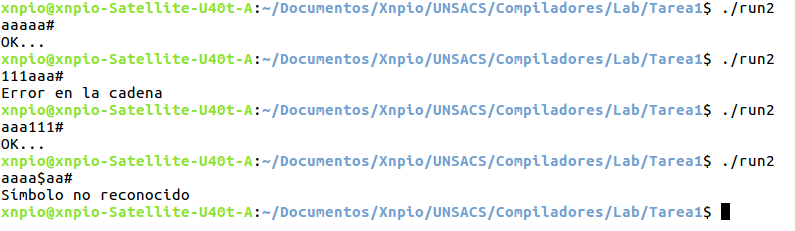
\includegraphics[scale = 0.5]{2.png}
\end{figure}



\end{enumerate}
\end{document}

